% Work-MAT | 2. rocnik | pripravovana hodina 50
% Návaznost: uživatelské připravy.zip (hodiny 01–20), autorská učebnice na GitHubu.
% Realisticky.cz: didaktická inspirace v posloupnosti a typech úloh; zadání jsou vlastní.
\documentclass[11pt,a4paper]{article}
\input{../../sablony/pripravy/priprava.sty}
\usepackage{tikz}
\nastavPripravu{2. ročník}{Goniometrické funkce}{50}{Sinus a kosinus obecného úhlu}
\begin{document}
\blok{Motivace a návaznost}
Vrať se na jednotkovou kružnici: bod koncového ramene úhlu má souřadnice $(\cos\alpha;\sin\alpha)$. Připomeň kvadranty a znaménka.
\poznamka{Orientační nabídka pro 45--55 minut: krátké zopakování a motivace, nový výklad, tři společné vzorové úlohy, samostatná práce. Vyber podle tempa třídy; zbývající zadání slouží jako rezerva.}
\blok{Výklad}
Sinus orientovaného úhlu je druhá souřadnice bodu na jednotkové kružnici, kosinus první. Platí $-1\le\sin\alpha,\cos\alpha\le1$.
\begin{center}
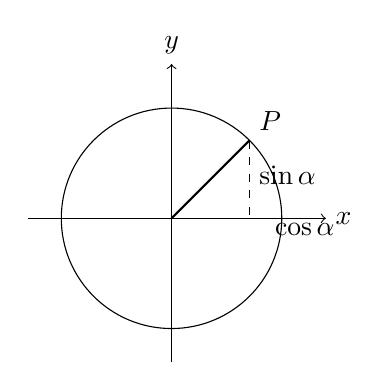
\begin{tikzpicture}[scale=1.4]
\draw[->] (-1.3,0)--(1.4,0) node[right] {$x$};
\draw[->] (0,-1.3)--(0,1.4) node[above] {$y$};
\draw (0,0) circle (1);
\draw[thick] (0,0)--(0.7071,0.7071);
\draw[dashed] (0.7071,0.7071)--(0.7071,0);
\node[above right] at (0.7071,0.7071) {$P$};
\node[below right] at (0.85,0.04) {$\cos\alpha$};
\node[right] at (0.7071,0.39) {$\sin\alpha$};
\end{tikzpicture}
\end{center}
\blok{Společné příklady}
\begin{prikladReseniBox}[title={Příklad 1}]
Vyřeš, resp. urči: $\sin150^\circ,\quad\cos150^\circ$.
\tcblower
\[\begin{aligned}\sin150^\circ=\frac{1}{2} \\ \cos150^\circ=-\frac{\sqrt3}{2}\end{aligned}\]
\end{prikladReseniBox}
\begin{prikladReseniBox}[title={Příklad 2}]
Vyřeš, resp. urči: $\sin240^\circ,\quad\cos240^\circ$.
\tcblower
\[\begin{aligned}\sin240^\circ=-\frac{\sqrt3}{2} \\ \cos240^\circ=-\frac{1}{2}\end{aligned}\]
\end{prikladReseniBox}
\poznamka{Před výpočtem konkrétních hodnot vždy určete kvadrant a znaménko.}
\blok{Samostatné procvičování}
\begin{zadaniReseniBox}[title={Samostatná práce 1}]
\begin{enumerate}[label=\alph*)]
\item $\operatorname{tg}60^\circ$.
\item $\operatorname{cotg}60^\circ$.
\item $\sin330^\circ$.
\item $\cos300^\circ$.
\item $\sin270^\circ$.
\item $\cos180^\circ$.
\end{enumerate}
\tcblower
\begin{enumerate}[label=\alph*)]
\item $\sqrt3$.
\item $\frac{\sqrt3}{3}$.
\item $-\frac{1}{2}$.
\item $\frac{1}{2}$.
\item $-1$.
\item $-1$.
\end{enumerate}
\end{zadaniReseniBox}
\blok{Dobrovolné rozšíření}
\begin{zadaniReseniBox}[title={Rozšíření 1}]
\begin{enumerate}[label=\alph*)]
\item Navrhni obdobnou úlohu s jiným úhlem a zkontroluj výsledek graficky..
\end{enumerate}
\tcblower
\begin{enumerate}[label=\alph*)]
\item $Srovnej s jednotkovou kružnicí nebo grafem.$.
\end{enumerate}
\end{zadaniReseniBox}
\blok{Úkol na doma}
Každou hodnotu zdůvodni náčrtkem jednotkové kružnice nebo orientovaným úhlem; u přesných hodnot neuváděj jen desetinné aproximace.
\begin{zadaniReseniBox}[title={Domácí úkol}]
\begin{enumerate}[label=\alph*)]
\item $\operatorname{tg}45^\circ$.
\item $\sin0^\circ$.
\item $\operatorname{cotg}135^\circ$.
\item $\sin60^\circ$.
\item $\sin30^\circ$.
\item $\cos60^\circ$.
\item $\sin45^\circ$.
\item $\cos45^\circ$.
\end{enumerate}
\tcblower
\begin{enumerate}[label=\alph*)]
\item $1$.
\item $0$.
\item $-1$.
\item $\frac{\sqrt3}{2}$.
\item $\frac{1}{2}$.
\item $\frac{1}{2}$.
\item $\frac{\sqrt2}{2}$.
\item $\frac{\sqrt2}{2}$.
\end{enumerate}
\end{zadaniReseniBox}
\poznamka{Domácí úkol obsahuje 8 položek; předpokládaná domácí práce přibližně 15--30 minut. Po větších blocích jsou vědomě promíchané dříve probrané typy.}
\end{document}
